\documentclass{article}
\usepackage{amsmath}
\usepackage{mathtools}
\usepackage{amssymb}
\usepackage{algorithm2e}
\usepackage{booktabs}
\usepackage{todonotes}
\usepackage{subfig}

\newcommand{\eqn}[1]{
	\begin{equation*}
		#1
	\end{equation*}
}

\newcommand{\eqna}[1]{
	\begin{eqnarray*}
		#1
	\end{eqnarray*}
}

\newcommand{\missing}[1]{
	\rule{0.8\textwidth}{.5pt}

	\dots\dots\dots\dots\dots\dots\dots

	#1

	\dots\dots\dots\dots\dots\dots\dots

	\rule{0.8\textwidth}{.5pt}
}


\usepackage{graphicx}
\graphicspath{{images/}}
\DeclareGraphicsExtensions{.pdf,.png,.jpg}

\newcommand{\img}[4]{
	% #1 - source
	% #2 - label
	% #3 - caption
	% #4 width, relative to \textwidth
	\begin{figure}[!t]
		\centering
		\includegraphics[width=#4\textwidth]{#1}
		\caption{#3}
		\label{#2}
	\end{figure}
}

\newcommand{\imgs}[8]{
	\begin{figure}[!tbh]
		\begin{minipage}[b]{#4\textwidth}
			\centering
			\includegraphics[width=\textwidth]{#1}
			\caption{#3}
			\label{#2}
		\end{minipage}
		\hfill
		\begin{minipage}[b]{#8\textwidth}
			\centering
			\includegraphics[width=\textwidth]{#5}
			\caption{#7}
			\label{#6}
		\end{minipage}
	\end{figure}
}

\begin{document}




\section{Definitions and Notation}


% undirected, simple graph
A \emph{graph} $G = (V,E)$ is an ordered pair of \emph{vertices} $V = \{v_1, v_2, \dots v_{|V|}\}$ and \emph{edges} $E$.
Here, we only consider \emph{undirected graphs without loops}, i.e., $E \subseteq \{\{v,w\}: v,w \in V, v \neq w\}$.
% connected graph
Two vertices $v$ and $w$ are called \emph{connected} in case there exists a path between them.
A graph is called \emph{connected} in case any pair of vertices $(v,w)$ is connected.
% subgraph
For a subset $V'$ of the vertex set $V$, we refer to $G^{V'} = (V', E'), E' := \{\{v,w\} \in E : v, w \in V'\}$ as the $V'$-induced subgraph of $G$.

% k-neighborhood
As the \emph{k-Neighborhood} $N_k(e)$ of an edge $e = \{a,b\}$, we denote the set of all $(k-2)$-tuples of vertices $v \in V, a \neq v \neq b$ that are connected to vertices $a$ or $b$ in the induced subgraph.
We call each element $N \in N_k(e)$ a \emph{neighbor set} of $e$.
Each of them corresponds to the subgraph $G^{\{a,b\} \cup N}$ of $G$ that contains $a$ and $b$ as well as $k-2$ other vertices.

% adjacency matrix
For a graph $G$, its \emph{adjacency matrix} $A(G) = A_{i,j}$ is an $n \times n$ matrix defined as follows:

\eqn{
A^u_{ij} =
	\left\{ \begin{array}{rl}
		1 \text{ (true)} & \text{if } i > j \land \{v_i,v_j\} \in E \\
		0 \text{ (false)} & \text{if } i > j \land \{v_i,v_j\} \notin E \\
		\text{undefined} & \text{otherwise}
	\end{array} \right.
}

We denote the \emph{set of all adjacency matrices} of size $k$ as ${\cal A}_k$, $|{\cal A}_k| = 2^{\frac{n \cdot (n-1)}{2}}$.
The set of the adjacency matrices of \emph{connected graphs} of size $k$ is denoted as ${\cal A}_k^{con} \subset {\cal A}_k$.
As examples consider the following adjacency matrices:

\begin{figure}[!htb]
\centering
\scriptsize
\subfloat[$G_i, |E_i| = 3, n(G_i) = 22$]{\begin{minipage}[b]{.3\textwidth}
	\centering
	\begin{tabular}{r|cccc}
	&	0	&	1	&	2	&	3	\\
\hline
0	&	-	&	0	&	1	&	1	\\
1	&		&	-	&	0	&	1	\\
2	&		&		&	-	&	0	\\
3	&		&		&		&	-	\\
\end{tabular}

	\resizebox {1.0\textwidth} {!} { \begin{tikzpicture}
\def \radius {3cm}
\draw (90:3) node[circle,draw] (v0) {0};
\draw (0:3) node[circle,draw] (v1) {1};
\draw (270:3) node[circle,draw] (v2) {2};
\draw (180:3) node[circle,draw] (v3) {3};
\path[-] (v0) edge [thick]  (v2);
\path[-] (v0) edge [thick]  (v3);
\path[-] (v1) edge [thick]  (v3);
\end{tikzpicture}
 }
\end{minipage}}
\hfill
\subfloat[$G_j, |E_j| = 3, n(G_j) = 49$]{\begin{minipage}[b]{.3\textwidth}
	\centering
	\begin{tabular}{r|cccc}
	&	0	&	1	&	2	&	3	\\
\hline
0	&	-	&	1	&	0	&	0	\\
1	&		&	-	&	0	&	1	\\
2	&		&		&	-	&	1	\\
3	&		&		&		&	-	\\
\end{tabular}

	\resizebox {1.0\textwidth} {!} { \begin{tikzpicture}
\def \radius {3cm}
\draw (90:3) node[circle,draw] (v0) {0};
\draw (0:3) node[circle,draw] (v1) {1};
\draw (270:3) node[circle,draw] (v2) {2};
\draw (180:3) node[circle,draw] (v3) {3};
\path[-] (v0) edge [thick]  (v1);
\path[-] (v1) edge [thick]  (v3);
\path[-] (v2) edge [thick]  (v3);
\end{tikzpicture}
 }
\end{minipage}}
\hfill
\subfloat[$G_k, |E_k| = 5, n(G_k) = 59$]{\begin{minipage}[b]{.3\textwidth}
	\centering
	\begin{tabular}{r|cccc}
	&	0	&	1	&	2	&	3	\\
\hline
0	&	-	&	1	&	1	&	0	\\
1	&		&	-	&	1	&	1	\\
2	&		&		&	-	&	1	\\
3	&		&		&		&	-	\\
\end{tabular}

	\resizebox {1.0\textwidth} {!} { \begin{tikzpicture}
\def \radius {3cm}
\draw (90:3) node[circle,draw] (v0) {0};
\draw (0:3) node[circle,draw] (v1) {1};
\draw (270:3) node[circle,draw] (v2) {2};
\draw (180:3) node[circle,draw] (v3) {3};
\path[-] (v0) edge [thick]  (v1);
\path[-] (v0) edge [thick]  (v2);
\path[-] (v1) edge [thick]  (v2);
\path[-] (v1) edge [thick]  (v3);
\path[-] (v2) edge [thick]  (v3);
\end{tikzpicture}
 }
\end{minipage}}
\caption{Examples of connected 4-vertex graphs}
\end{figure}

% adjacency matrix key
Assume $a$ to be the sequence of all defined entries of an adjacency matrix $A$, i.e., $a = (a_1, a_2, \dots a_{\frac{k \cdot (k-1)}{2}}) := (A_{1,2}, A_{1,3}, \dots A_{k-1,k})$
Then, we define the \emph{key} of an adjacency matrix $A$ and the corresponding graph $G$ as follows:

\eqn{n(A) = n(G) := \sum_{i=1}^{\frac{k \cdot (k-1)}{2}} a_i \cdot 2^{i-1}}

% set of all adjacency matrix keys, set of all connected adjacency matrix keys
Then, ${\cal N}_k^{con} \subset [0,2^{\frac{k \cdot (k-1)}{2}}]$ denotes the set of all keys of connected graphs of size $k$.


% dynamic graph and updates
As a dynamic graph, we consider a graph whose set of edges $E$ changes over time.
We assume that in each time step, a single edge is either added to or removed from $E$.
This change is denoted as an update: either $add(e)$ or $rm(e)$.
A graph is transformed from $G_i$ to $G_{i+1}$ by the application of update $u_{i+1}$.
\todo{add example of graph transformation over time...}



% % adjacency matrix
% An \emph{adjacency matrix} $A$ is the $n \times n$ matrix representation of a graph $G=(V,E)$ with $n := |V|$.
% As we are only considering undirected graphs without loops, the diagonal values are all undefined and all other values mirrored, i.e., $A_{i,i} := -, i \in [1, |V|]$ and $A_{i,j} := A_{j,i}$.
% We denote the adjacency matrix of the $V'$-induced subgraph $G'$ of $G$ as $A^{V'}$.

% $A$ can be represented as a sequence $a(A)$ of length $\frac{n \cdot (n-1)}{2}$, defined as follows:

% \eqn{a(A) := (A_{1,2}, A_{1,2}, \dots A_{1,n}, A_{2,3}, A_{2,4}, \dots A_{n-1,n})}

% Therefore, all possible adjacency matrices for a given graph size $n$ can be represented as the set ${\cal A}^n = \{0,1\}^{\frac{n \cdot (n-1)}{2}}$.
% We refer to ${\cal A}^n_{con} \subset {\cal A}^n$ as the set of all connected adjacency matrices of size $n$, i.e., there exists a path between any pair of vertices $(v,w), v, w \in V$.
% As examples, consider the boolean sequence representation for 3-, 4-, and 5-vertex graphs:

% \eqna{
% 	3: && a(A \in {\cal A}^3) = (A_{1,2}, A_{1,3}, A_{2,3}) \\
% 	4: && a(A \in {\cal A}^4) = (A_{1,2}, A_{1,3}, A_{1,4}, A_{2,3}, A_{2,4}, A_{3,4}) \\
% 	5: && a(A \in {\cal A}^5) = (A_{1,2}, A_{1,3}, A_{1,4}, A_{1,5}, A_{2,3}, A_{2,4}, A_{2,5}, A_{3,4}, A_{3,5}, A_{4,5})
% }

% Each element $a$ from this set can also be interpreted as a number $n(a) \in \mathbb{N}$ as follows:

% \eqn{n(a \in {\cal A}^n) = \sum_{i=1}^{\frac{n \cdot (n-1)}{2}} 2^{i-1} \cdot a_i}

% Using this assignment, we can represent adjacency matrices as simple numbers $n(A) := n(a(A))$ referred to as its key.




\section{Motifs}

As motifs of size $k$, also called $k$-vertex motifs or $k$-motifs, we consider the equivalence classes of isomorph connected k-vertex graphs which we denote as ${\cal M}_k$.

Therefore, each connected adjacency matrix $A \in {\cal A}_k^{con}$ is element of exactly one equivalence class represented by a motif $m \in {\cal M}_k$.
We express this property as a function that maps the key $n(A)$ of a connected adjacency matrix $A$ to a motif $m \in M_k$, i.e.,

\eqn{r : {\cal N}_k^{con} \rightarrow {\cal M}_k}

This assignment can be computed by enumerating all connected adjacency matrices and determining their equivalence class by performing an isomorphism check with all existing motifs.

\begin{figure}[!htb]
	\subfloat[3-vertex motifs: ${\cal M}_3$]{
	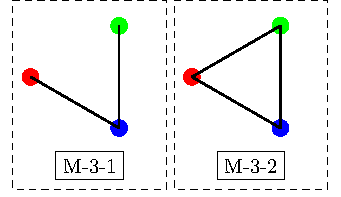
\includegraphics[width=.38\textwidth]{m-3}
	}
	\hfill
	\subfloat[4-vertex motifs: ${\cal M}_4$]{
	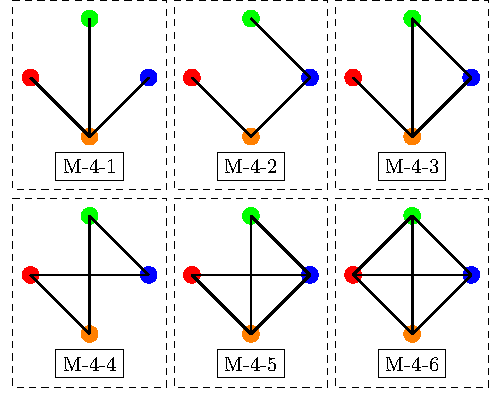
\includegraphics[width=.58\textwidth]{m-4}
	}
	\caption{Examples for the set of motifs ${\cal M}_k$ for different sizes}
\end{figure}



\section{Implementation}

For simplicity, we store the function $r$ as integer pairs $(n,m)$ where $n$ is the key of a connected adjacency matrix and $m$ the index of the equivalence class, or motif, it belongs to.










\section{Algorithm}


\newcommand{\mcount}{{\cal F}}
\newcommand{\mcountof}[1]{{\cal F}(\motif{#1})}
\newcommand{\mcountofat}[2]{{\cal F}_{#2}(\motif{#1})}

\newcommand{\operation}{{\cal O}}
\newcommand{\signature}{{\cal S}}
\newcommand{\signatureofabcd}{\signature(a,b,c,d)}

Whenever an edge $e = \{a,b\}$ is added to or removed from a graph $G_i$, each subgraph $G_i^{\{a,b\} \cup N}, N \in N_k(e)$ represents a motif that is created, transformed, or dissolved.

In case $u_i = rm(e)$, $n(A_i^{\{a,b\} \cup N})$ is the key of the adjacency matrix for $N \in N_k(e)$ before the removal.
After the removal, the key will be $n(A_{i+1}^{\{a,b\} \cup N}) = n(A_i^{\{a,b\} \cup N})-1$, i.e., the same adjacencies except for the missing edge between the first two vertices.
If $n(A_i^{\{a,b\} \cup N})-1 \notin {\cal N}_k^{con}$, the existing motif will be dissolved and is transformed otherwise.

Similarly, in case $e$ is added to the graph $G_i$, $n(A_{i+1}^{\{a,b\} \cup N}) = n(A_i^{\{a,b\} \cup N})+1$ is the key of the adjacency matrix for the neighbor set $N \in N(a,b)$ afterwards.
If $n(A_i^{\{a,b\} \cup N}) \notin {\cal N}_k^{con}$, a new motif is created and an existing one transformed otherwise.

From this, we can define an algorithm that updates the motif frequency ${\cal F}$ for the application of an update $u_i$.
In addition, all changes to motifs in the graph can be listed:

\begin{algorithm}[!htb]
	\KwData{$G_i, e = \{a,b\}, type \in \{add, rm\}, print \in \{true, false\}$}
	\SetKwComment{Comment}{/* }{ */}
	\Begin{
		\For{$N \in N_k(e)$}{
			$n_{i} = n(A_i^{\{a,b\} \cup N})$
			\Comment*[r]{key before}
			\uIf{$type = add$}{
				$n_{i+1} = n_{i} + 1$
				\Comment*[r]{key after addition}
			}
			\uElse{
				$n_{i+1} = n_{i} - 1$
				\Comment*[r]{key after removal}
			}

			\uIf{$n_{i} \in {\cal N}_k^{con}$}{
				${\cal F}(r(n_{i})) -= 1$ \Comment*[r]{decr old motif}
			}
			\uIf{$n_{i+1} \in {\cal N}_k^{con}$}{
				${\cal F}(r(n_{i+1})) += 1$ \Comment*[r]{incr new motif}
			}

			\uIf{print}{
				\uIf{$n_{i} \in {\cal N}_k^{con} \land n_{i+1} \in {\cal N}_k^{con}$}{
					print `transformed: a, b, N ($r(n_{i}) \rightarrow r(n_{i+1})$)'
				}
				\uElseIf{$n_{i} \in {\cal N}_k^{con}$}{
					print `dissolved: a, b, N ($r(n_{i})$)'
				}
				\uElse{
					print `created: a, b, N ($r(n_{i+1})$)'
				}
			}
		}
	}
	\caption{\emph{StreaM$_k$} for maintaining $\mcount$ in dynamic graphs}
	\label{alg:u}
\end{algorithm}




\section{Complexity of Algorithm}

\todo{define $d_{max}$ here?!?}

When processing an update $u_{i+1}$, i.e., $add(\{a,b\})$ or $rm(\{a,b\})$, we must iterate over all elements of $N_k(a,b)$ with $|N_k(a,b)| \leq d_{max}^{k-2}$.
Processing each neighborhood $N \in N_k(a,b)$ can be done in $O(1)$ as it only requires the generation of the key $n(A^{\{a,b\} \cup N})$, its lookup in the pre-computed assignment $r$, and the adaptation of ${\cal F}$.
Therefore, the complexity for the execution of the algorithms is $O(d_{max}^{k-2})$.








\section{Statistics about motifs}

\begin{table}[!h]
\centering
\begin{tabular}{c rrr rrr}
\toprule
$k$						& 2		& 3		& 4		& 5		& 6			& 7 \\
\midrule
$|{\cal A}_k|$			& 2		& 8		& 64	& 1,024	& 32,768	& 2,097,152 \\
$|{\cal A}_k^{con}|$ 	& 1		& 4		& 38	& 827	& 26,704	& 1,866,256 \\
$|{\cal M}_k|$			& 1		& 2		& 6		& 21	& 112		& 853 \\
\bottomrule
\end{tabular}
\caption{Statistics about adjacency matrices and motifs of different sizes}
\end{table}


% \imgs{um-stats}{fig:um-stats}{stats of undirected motifs}{0.4}{um-stats-labeled}{fig:um-stats-labeled}{stats of undirected motifs}{0.4}





\end{document}